\paragraph*{Идентификация трения\\}%Трения чего?
\hspace*{\parindent}В предыдущих лабораторных работах были найдены параметры $J_m^1, K_e^1, K_m^1, R$ для мотора NXT. В данной лабораторной работе исследуется сочленение манипулятора, коэффициент редукции которого отличается от коэффициента мотора NXT в $i$ раз. Для нахождения новых значений параметров $J_m, K_e, K_m$ нужно вычислить значение коэффициента редукции $i$, разделив количество зубьев ведомой шестерни на количество зубьев ведущей. Затем, рассчитать новые параметры по формулам:
\begin{equation}
	J_m=J_m^1i^2, \phantom{-} K_e = K_e^1i, \phantom{-} K_m = K_m^1i,
\end{equation}

Для нахождения значения коэффициента трения воспользуемся методом наименьших квадратов. На вход системы будем подавать напряжение $u(t) = U_m\sin{{\omega}t}$, где $U_m$ - максимальное напряжение двигателя. Для аппроксимации функции необходимо решить дифференциальное уравнение \eqref{dif}. Его решением будет следующая функция:
\begin{equation}\label{theta}
	\theta(t)=\frac{B(A^2(1-\cos{{\omega}}t)+\omega^2(1-e^{-At})-A\omega\sin{{\omega}t)}}{A\omega(A^2+\omega^2)},
\end{equation}где $A=\frac{K_f}{J_m}+\frac{K_eK_m}{J_mR}$, $B=\frac{K_mU_m}{J_mR}$.

Считая $K_f = 0$, рассчитаем значения $A$ и $B$ и построим график при $u(t) = U_m\sin{2t}$, изображенный на рис.~\ref{nofr}.

\begin{figure}[h]
	\noindent\centering{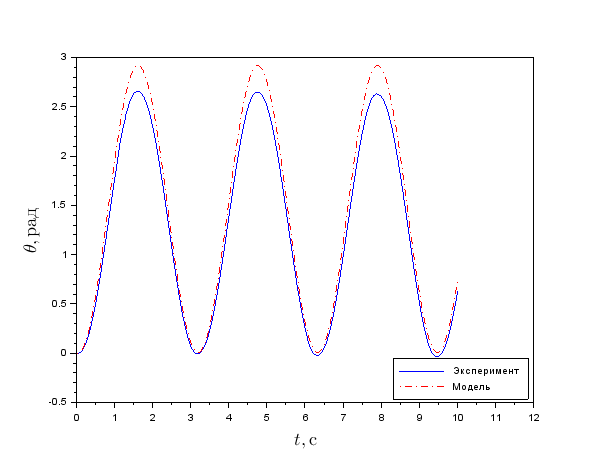
\includegraphics[height = 6cm]{img/sin2.png}}
	\caption{График модели без учета трения}
	\label{nofr}
\end{figure}

Аппроксимируем функцию \eqref{theta} по $A$ с помощью функции "datafit" пакета \textit{Scilab} и построим график, изображенный на рис.~ \ref{yesfr}. Так как $A$ зависит от неизвестного коэффициента $K_f$, то аппроксимирую функцию по $A$ мы учитываем $K_f$. %можем найти K_f

\begin{figure}[h]
	\noindent\centering{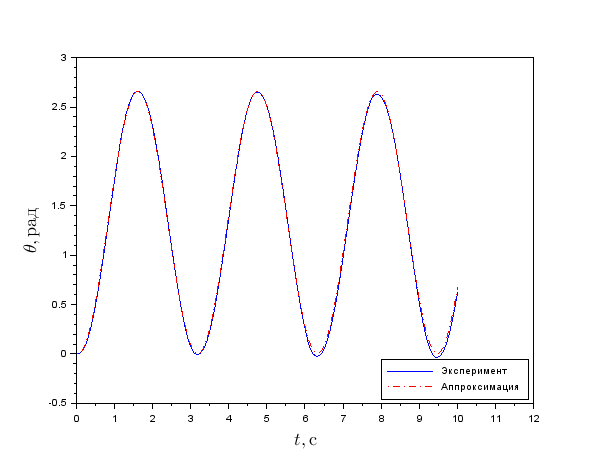
\includegraphics[height = 6cm]{img/kfsin2.png}}
	\caption{График модели с учетом трения}
	\label{yesfr}
\end{figure}

Очевидно, что введение коэффициента $K_f$ сделало математическую модель двигателя более правдоподобной.

Из полученного значения $A$ выведем:
\begin{equation}
	K_f = J_mA-\frac{K_eK_m}{R}, \phantom{-} K=J_mA,
\end{equation}

% Для чего учет трения